\documentclass[aspectratio=169]{beamer}
\usetheme{Madrid}
\usecolortheme{seahorse}
\usepackage{booktabs}
\usepackage{graphicx}
\usepackage{amsmath}
\usepackage{tikz}
\usetikzlibrary{arrows.meta,positioning,calc}

% all images copied locally — one path is enough
\graphicspath{{./}}

\title{PEM Fuel Cell Stack Modelling \& Parameter Tuning}
\subtitle{From physical principles to per-cell calibration}
\author[LAGHA Khalil]{%
    \textbf{LAGHA Khalil}\\[0.3em]
    {\small Supervisor: Emmanuel Witrant}
}
\institute[GIPSA-lab / UGA]{%
    GIPSA-lab — Université Grenoble Alpes
}
\date{May 2026}

\begin{document}

% ── Title frame with logos ────────────────────────────────────────────────────
\begin{frame}
    \begin{tikzpicture}[remember picture, overlay]
        \node[anchor=north west, inner sep=8pt] at (current page.north west)
            {
\includegraphics[height=1.1cm]{UGAlogo.png}};
        \node[anchor=north east, inner sep=8pt] at (current page.north east)
            {
\includegraphics[height=1.1cm]{gipsa-lablogo.jpg}};
    \end{tikzpicture}
    \titlepage
\end{frame}

% ── Outline ───────────────────────────────────────────────────────────────────
\begin{frame}{Outline}
    \tableofcontents
\end{frame}

% ─────────────────────────────────────────────────────────────────────────────
\section{Physical Principle}

\begin{frame}{Operating Principle of a PEM Fuel Cell}
    \begin{columns}
        \column{0.55\textwidth}
        \begin{itemize}
            \item \textbf{Anode:} $\mathrm{H_2 \rightarrow 2H^+ + 2e^-}$
            \item \textbf{Cathode:} $\mathrm{\frac{1}{2}O_2 + 2H^+ + 2e^- \rightarrow H_2O}$
            \item \textbf{Overall:} $\mathrm{H_2 + \frac{1}{2}O_2 \rightarrow H_2O + electricity + heat}$
            \item Proton Exchange Membrane (PEM) conducts \(\mathrm{H^+}\), blocks electrons
            \item Water management critical: too dry → conductivity loss; flooding → transport blockage
        \end{itemize}
        \column{0.45\textwidth}
        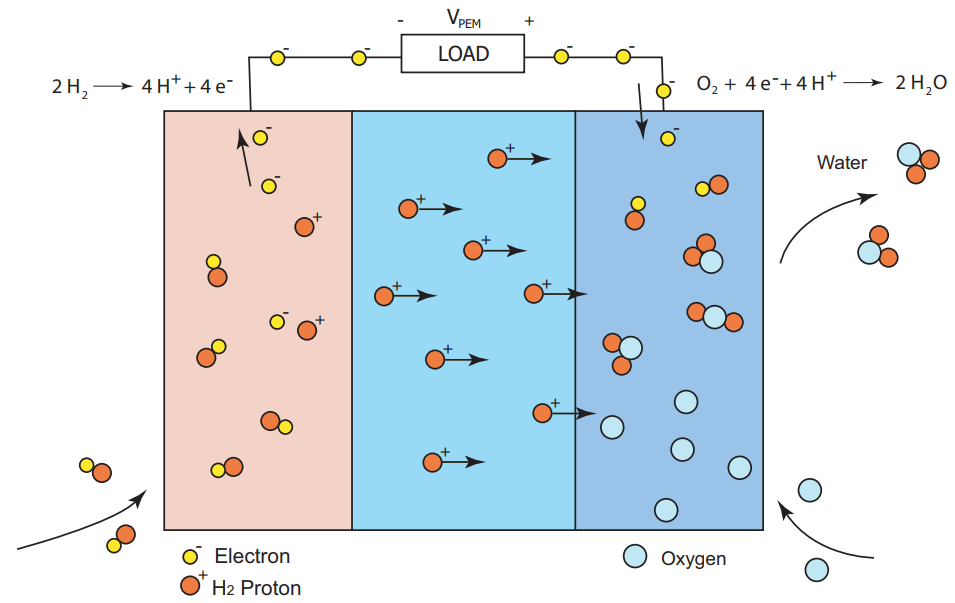
\includegraphics[width=\linewidth]{Capture d'écran 2026-04-15 143548.png}
    \end{columns}
\end{frame}

\begin{frame}{Voltage Losses — Polarisation Curve}
    \begin{columns}
        \column{0.5\textwidth}
        \begin{itemize}
            \item \textbf{Activation loss} — kinetic limitation at low current
            \item \textbf{Ohmic loss} — resistive drop, linear with current
            \item \textbf{Concentration loss} — mass-transport limit at high current
        \end{itemize}
        \vspace{0.5em}
        \[
            v_{fc} = E - v_\text{act} - v_\text{ohm} - v_\text{con}
        \]
        \column{0.5\textwidth}
        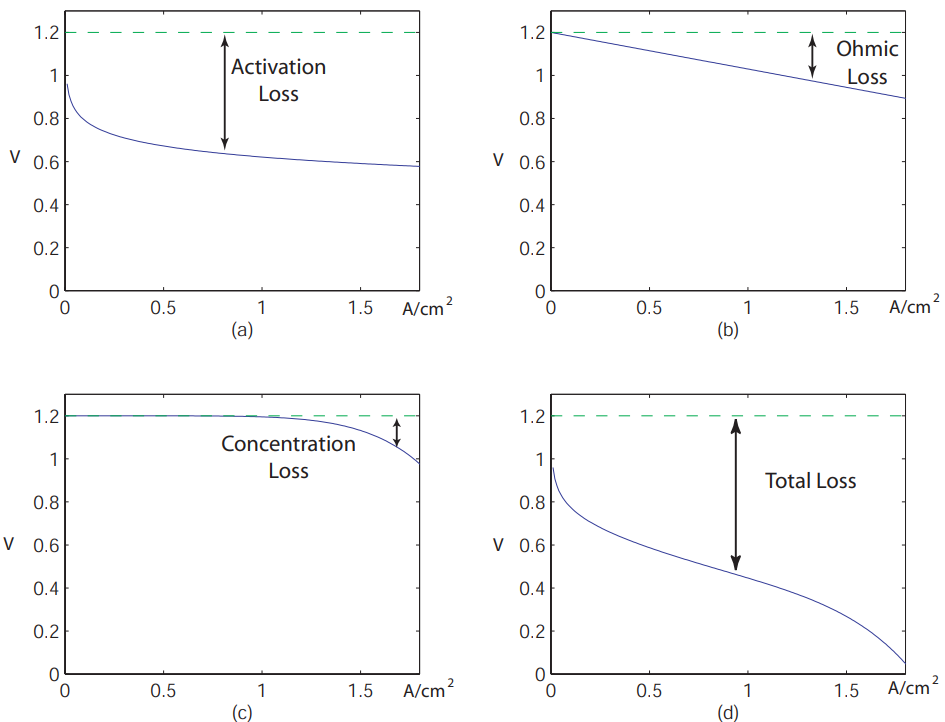
\includegraphics[width=\linewidth]{Capture d'écran 2026-04-17 100413.png}
    \end{columns}
\end{frame}

% ─────────────────────────────────────────────────────────────────────────────
\section{Single-Cell Model}

\begin{frame}{Open-Circuit Voltage (Nernst)}
    Derived from thermodynamics (Gibbs free energy, Faraday's law):
    \[
        E = 1.229 - 0.85\!\times\!10^{-3}(T-298.15)
          + 4.31\!\times\!10^{-5}\,T\!\left(\ln P_{H_2} + \tfrac{1}{2}\ln P_{O_2}\right)
    \]
    \begin{itemize}
        \item $1.229\,\mathrm{V}$ — standard reversible voltage at 25\,°C
        \item $-0.85\!\times\!10^{-3}$ — temperature coefficient from $\Delta S^0/2F$ (liquid water)
        \item Last term — Nernst pressure correction
    \end{itemize}
\end{frame}

\begin{frame}{Voltage Loss Equations}
    \begin{block}{Activation loss (kinetics)}
        \[
            v_\text{act} = \xi_1 + \xi_2 T + \xi_3 T\ln C_{O_2} + \xi_4 T\ln i_{FC}
        \]
    \end{block}
    \begin{block}{Ohmic loss (membrane resistance)}
        \[
            v_\text{ohm} = i_{FC}\!\left(\frac{t_m}{A_{fc}\,\sigma_m(\lambda_m, T)} + c\right),
            \qquad
            \sigma_m = (b_{11}\lambda_m - b_{12})\exp\!\left[b_2\!\left(\tfrac{1}{303}-\tfrac{1}{T}\right)\right]
        \]
    \end{block}
    \begin{block}{Concentration loss (mass transport)}
        \[
            v_\text{con} = -B\ln\!\left(1 - \frac{i_{FC}}{i_\text{max}}\right)
        \]
    \end{block}
    \textbf{Tuned per cell:} $\xi_1,\xi_2,\xi_3,\xi_4,\,B,\,c$ \quad
    \textbf{Fixed:} $T,\,P_{O_2}^*{=}0.21\,P_\text{atm},\,\lambda_m,\,A_{fc},\,t_m,\,i_\text{max}$
\end{frame}

\begin{frame}{Membrane Water Content — $\lambda_m$}
    Relative humidities are algebraic outputs of the water mass states:
    \[
        \phi_{an} = \frac{p_{v,an}}{p_{sat}(T)}, \qquad p_{v,an} = \frac{m_{w,an}\,R_v\,T}{V_{an}}
        \qquad
        \phi_{ca} = \frac{p_{v,ca}}{p_{sat}(T)}, \qquad p_{v,ca} = \frac{m_{w,ca}\,R_v\,T}{V_{ca}}
    \]
    Springer sorption isotherm converts activity $a\in[0,1]$ to water content:
    \[
        \lambda(a) = 0.043 + 17.81\,a - 39.85\,a^2 + 36.0\,a^3
    \]
    Membrane water content is the average of both sides:
    \[
        \lambda_m = \frac{\lambda(\phi_{an}) + \lambda(\phi_{ca})}{2}
    \]
    $\lambda_m$ then enters the membrane conductivity $\sigma_m$ and hence $v_{ohm}$.\\
    \textbf{Note:} in the simplified model $\lambda_m$ is held constant (e.g.\ $=14$) when water dynamics are not tracked.
\end{frame}

\begin{frame}{Subsystem Architecture}
    \begin{columns}
        \column{0.48\textwidth}
        Three coupled subsystems:
        \begin{itemize}
            \item \textbf{Anode} — hydrogen pressure $P_{H_2}$, anode humidity $\phi_{an}$
            \item \textbf{Membrane} — water transport (electro-osmotic drag + back-diffusion)
            \item \textbf{Cathode} — constant $P_{O_2}^*$, cathode humidity $\phi_{ca}$
        \end{itemize}
        \vspace{0.4em}
        All three feed into the \textbf{voltage block} to compute $v_{fc}$
        \column{0.52\textwidth}
        \resizebox{\linewidth}{!}{%
        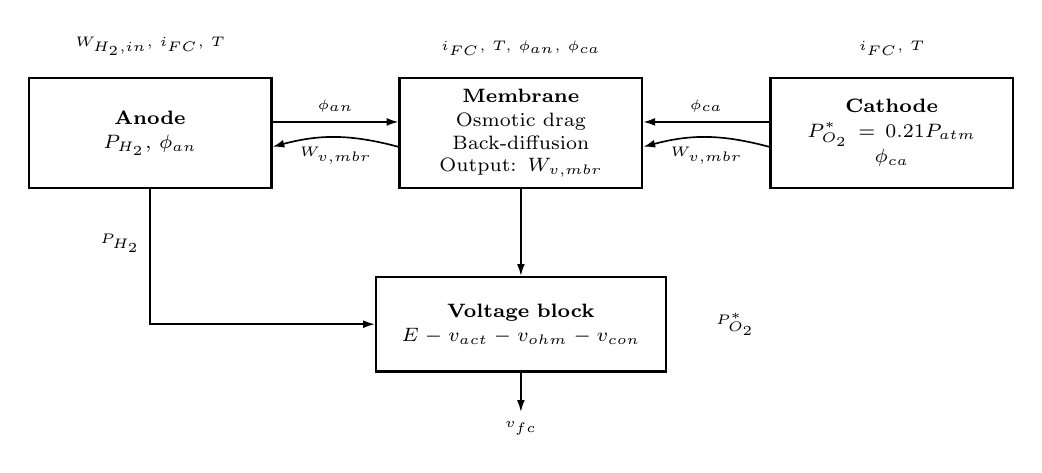
\begin{tikzpicture}[
            >=Latex,
            block/.style={draw,rectangle,thick,fill=white,align=center,
                          text width=2.8cm,minimum height=1.4cm,inner sep=4pt,font=\scriptsize},
            vblock/.style={draw,rectangle,thick,fill=white,align=center,
                           text width=3.4cm,minimum height=1.2cm,inner sep=4pt,font=\scriptsize},
            lab/.style={font=\tiny,align=center},
            line/.style={-{Latex[length=1.5mm,width=1mm]},line width=0.6pt}
        ]
        \node[block] (anode) {\textbf{Anode}\\[0.1em]
            $P_{H_2},\,\phi_{an}$};
        \node[block, right=1.6cm of anode] (membrane) {\textbf{Membrane}\\[0.1em]
            Osmotic drag\\Back-diffusion\\Output: $W_{v,mbr}$};
        \node[block, right=1.6cm of membrane] (cathode) {\textbf{Cathode}\\[0.1em]
            $P_{O_2}^*=0.21P_{atm}$\\$\phi_{ca}$};
        \node[vblock, below=1.1cm of membrane] (voltage) {\textbf{Voltage block}\\[0.1em]
            $E-v_{act}-v_{ohm}-v_{con}$};
        % inputs
        \node[lab,above=0.15cm of anode]{$W_{H_2,in},\,i_{FC},\,T$};
        \node[lab,above=0.15cm of membrane]{$i_{FC},\,T,\,\phi_{an},\,\phi_{ca}$};
        \node[lab,above=0.15cm of cathode]{$i_{FC},\,T$};
        % phi arrows
        \draw[line] ([yshift=4pt]anode.east) -- node[above,lab]{$\phi_{an}$} ([yshift=4pt]membrane.west);
        \draw[line] ([yshift=4pt]cathode.west) -- node[above,lab]{$\phi_{ca}$} ([yshift=4pt]membrane.east);
        % W_v,mbr arrows (cathode->membrane->anode)
        \draw[line] ([yshift=-5pt]membrane.west) to[bend right=15]
            node[below,lab]{$W_{v,mbr}$} ([yshift=-5pt]anode.east);
        \draw[line] ([yshift=-5pt]cathode.west) to[bend right=15]
            node[below,lab]{$W_{v,mbr}$} ([yshift=-5pt]membrane.east);
        % voltage block
        \draw[line] (anode.south) |- node[pos=0.2,left,lab]{$P_{H_2}$} (voltage.west);
        \draw[line] (membrane.south) -- (voltage.north);
        \node[lab,right=0.5cm of voltage]{$P_{O_2}^*$};
        \draw[line] (voltage.south) -- ++(0,-0.5) node[below,lab]{$v_{fc}$};
        \end{tikzpicture}%
        }
    \end{columns}
\end{frame}

% ─────────────────────────────────────────────────────────────────────────────
\section{State-space representation}

\begin{frame}{State-Space Representation}
    \[
        \dot{\mathbf{x}} = A\mathbf{x} + B\mathbf{u}, \qquad y = C\mathbf{x} + D\mathbf{u}
    \]
    \vspace{-0.3em}
    \[
        \mathbf{x} = \begin{bmatrix}P_{H_2}\\m_{w,an}\\m_{w,ca}\end{bmatrix},\quad
        \mathbf{u} = \begin{bmatrix}i_{FC}\\W_{H_2,in}\end{bmatrix},\quad
        y = v_{fc}
    \]
    \vspace{-0.2em}
    \begin{columns}
        \column{0.5\textwidth}
        \[
        A = \begin{bmatrix}
            -\dfrac{k_{an}R_{H_2}T}{V_{an}} & 0 & 0 \\[8pt]
            0 & -\dfrac{D_w}{V_{an}t_m} & \dfrac{D_w}{V_{ca}t_m} \\[8pt]
            0 & \dfrac{D_w}{V_{an}t_m} & -\dfrac{D_w}{V_{ca}t_m}
        \end{bmatrix}
        \]
        \column{0.5\textwidth}
        \[
        B = \begin{bmatrix}
            -\dfrac{M_{H_2}nR_{H_2}T}{2FV_{an}} & \dfrac{R_{H_2}T}{V_{an}} \\[8pt]
            \dfrac{n_d M_v}{F} & 0 \\[8pt]
            \dfrac{(n-2n_d)M_v}{2F} & 0
        \end{bmatrix}
        \]
    \end{columns}
    \vspace{0.3em}
    {\small $C$, $D$: Jacobians of $v_{fc}$ w.r.t.\ $\mathbf{x}$ and $\mathbf{u}$ at the operating point}
\end{frame}

% ─────────────────────────────────────────────────────────────────────────────
\section{Experiment}

\begin{frame}{Experimental Setup — Inputs \& Outputs}
    \begin{columns}
        \column{0.45\textwidth}
        \textbf{Inputs (controlled):}
        \begin{itemize}
            \item H\textsubscript{2} valve opening (0--100\,\%)
            \item H\textsubscript{2} inlet pressure (gauge $\rightarrow$ absolute atm)
            \item H\textsubscript{2} and air mass flow rates
        \end{itemize}
        \vspace{0.4em}
        \textbf{Outputs (measured):}
        \begin{itemize}
            \item Individual cell voltages: $v_0 \ldots v_9$ [mV]
            \item Stack voltage $V_\text{stack}$ [V]
            \item Load current: $I = V_\text{stack}/25\,\Omega$ [A]
        \end{itemize}
        \column{0.55\textwidth}
        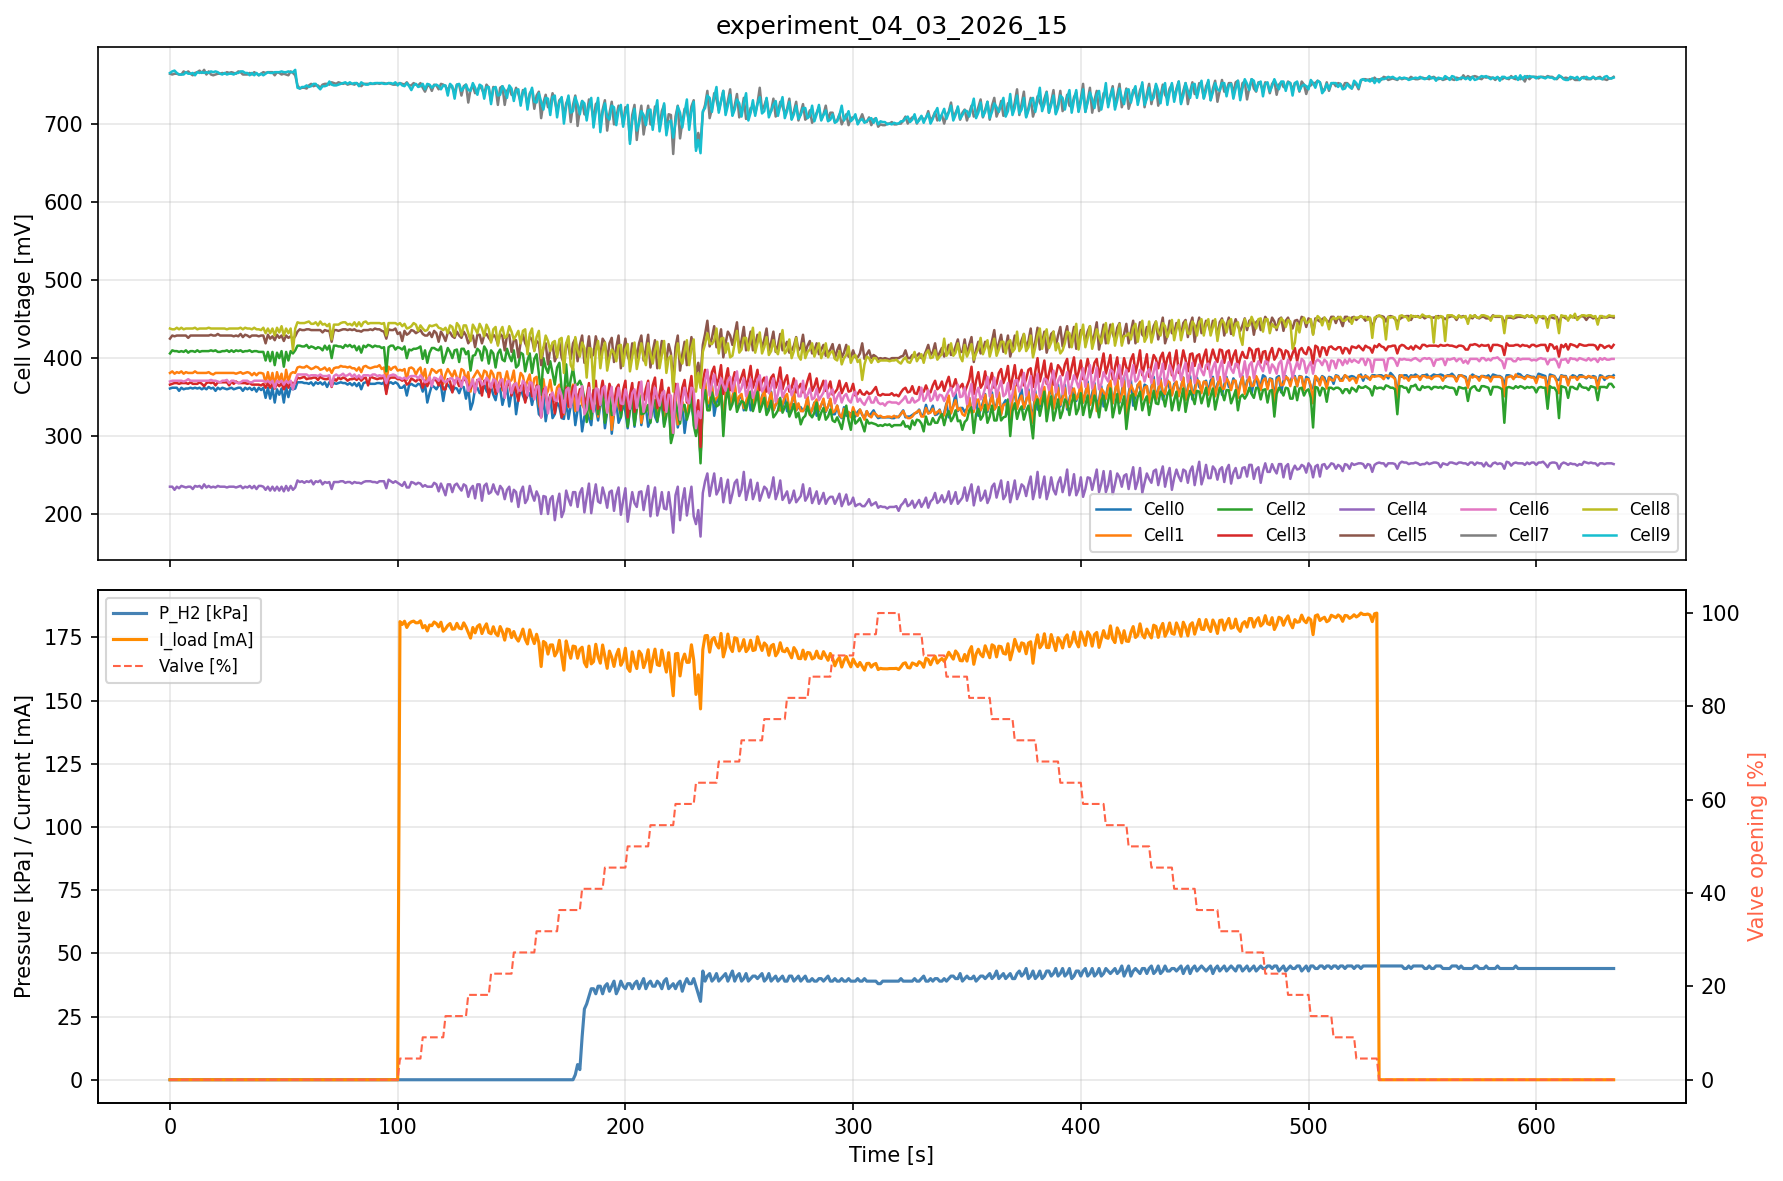
\includegraphics[width=\linewidth]{data_overview_experiment_04_03_2026_15.png}
    \end{columns}
\end{frame}

\begin{frame}{Experimental Setup — Experiment 19}
    \begin{columns}
        \column{0.45\textwidth}
        \textbf{Key difference vs Exp\,15:}
        \begin{itemize}
            \item \textbf{No valve control} — fixed 25\,$\Omega$ resistor connected at $t=135$\,s
            \item Resistor \textbf{removed} at $t=684$\,s — current returns to 0
            \item Current set by Ohm's law: $I = V_\text{stack}/R$ (loaded window only)
            \item Longer run: 1081\,s vs 635\,s
            \item Cells\,0,\,1,\,2\,\&\,8 drop to $\approx$\,0\,V under load (hardware degradation)
        \end{itemize}
        \column{0.55\textwidth}
        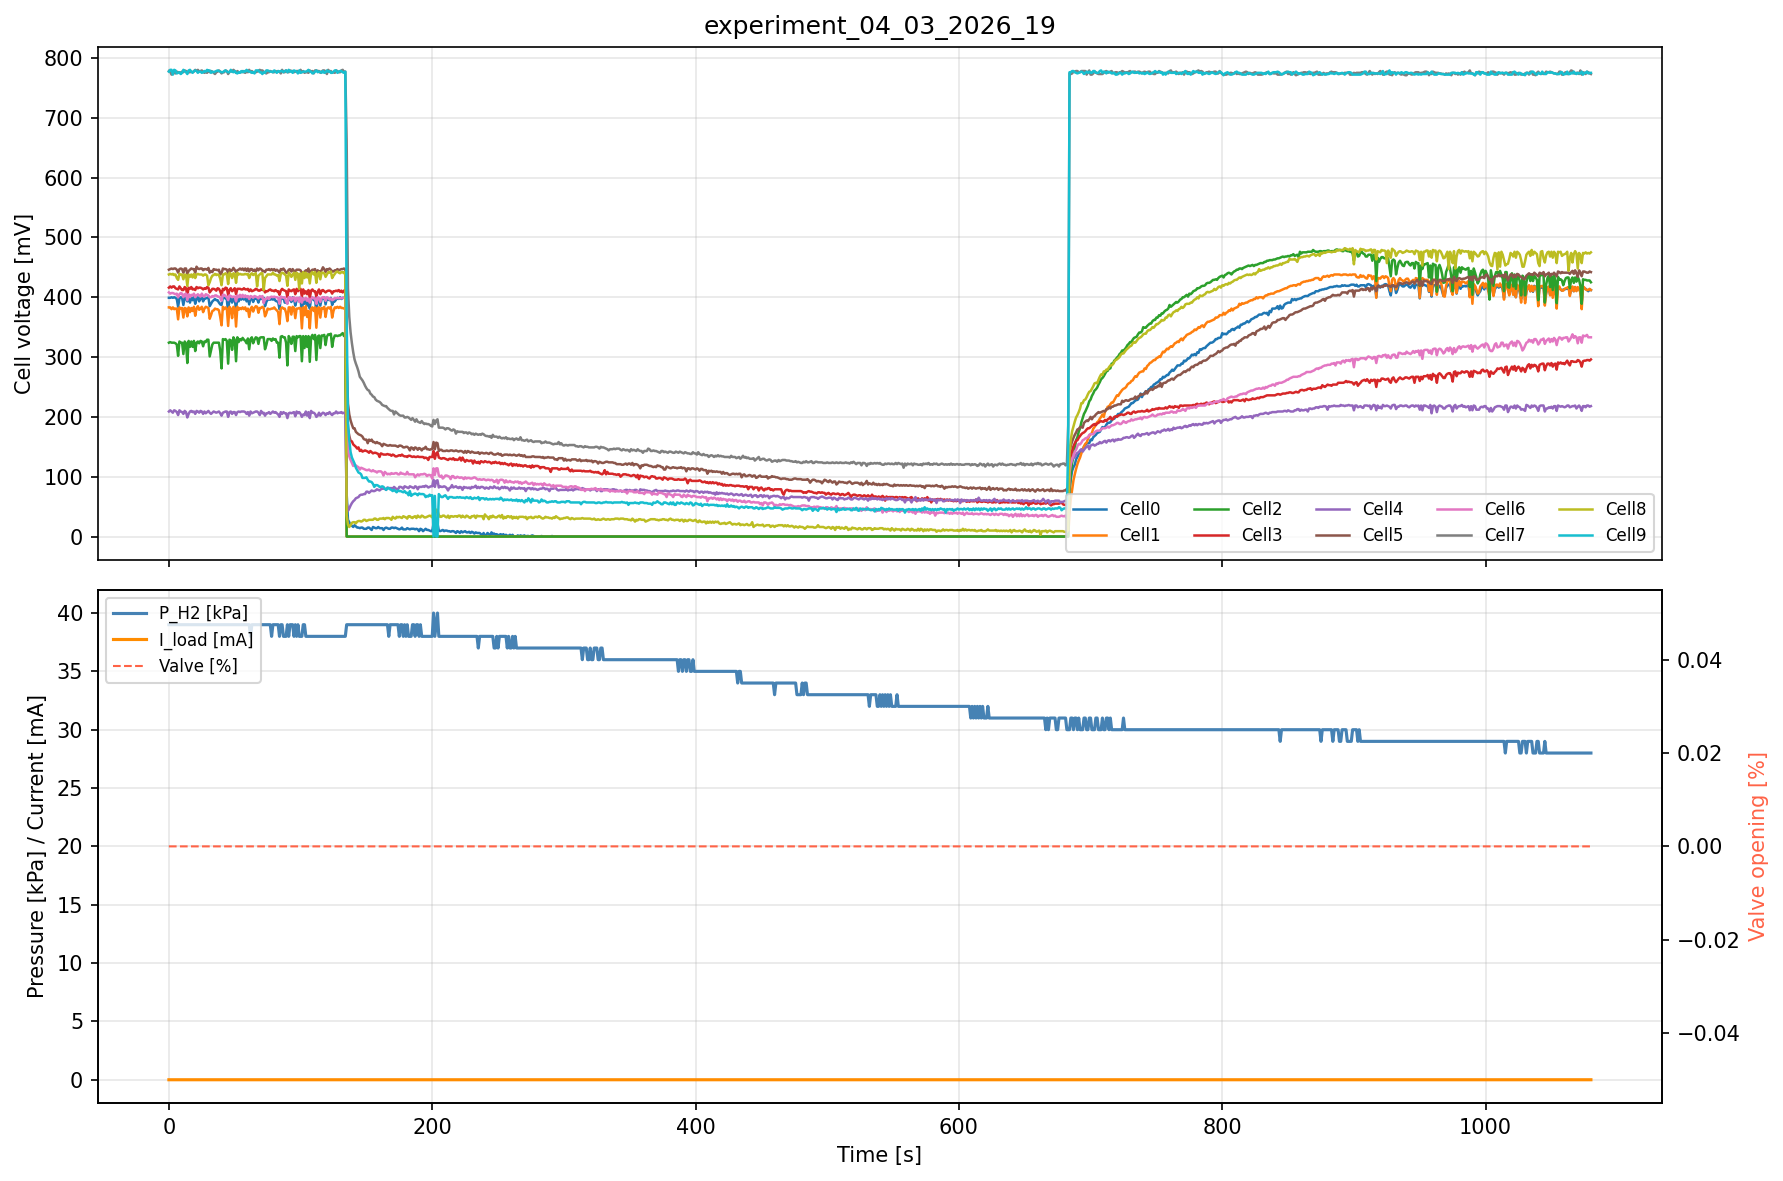
\includegraphics[width=\linewidth]{data_overview_experiment_04_03_2026_19.png}
    \end{columns}
\end{frame}

% ─────────────────────────────────────────────────────────────────────────────
\section{Optimization}

\begin{frame}{Two-Stage Per-Cell Optimisation}
    \textbf{Objective:} minimise RMSE between predicted and measured cell voltage
    \[
        \min_{\xi_1,\xi_2,\xi_3,\xi_4,B,c} \;\sqrt{\frac{1}{N}\sum_{i=1}^{N}\!\left(v_\text{model}(I_i, P_{H_2,i}) - v_\text{meas,i}\right)^2}
    \]
    \begin{enumerate}
        \item \textbf{Differential Evolution} (global) — population 20, max 800 generations, seed 42
        \item \textbf{L-BFGS-B} (local polish) — refines DE solution within bounds
    \end{enumerate}
    \vspace{0.3em}
    \textbf{Physical bounds enforced:}
    \begin{itemize}
        \item $\xi_4 \leq 0$ — activation loss increases with current
        \item $B \geq 0$ — concentration loss is always a drop
        \item $c \geq 0$ — ohmic resistance is always positive
    \end{itemize}
\end{frame}

% ─────────────────────────────────────────────────────────────────────────────
\section{Results}

\begin{frame}{Cost Evolution}
    \begin{columns}
        \column{0.5\textwidth}
        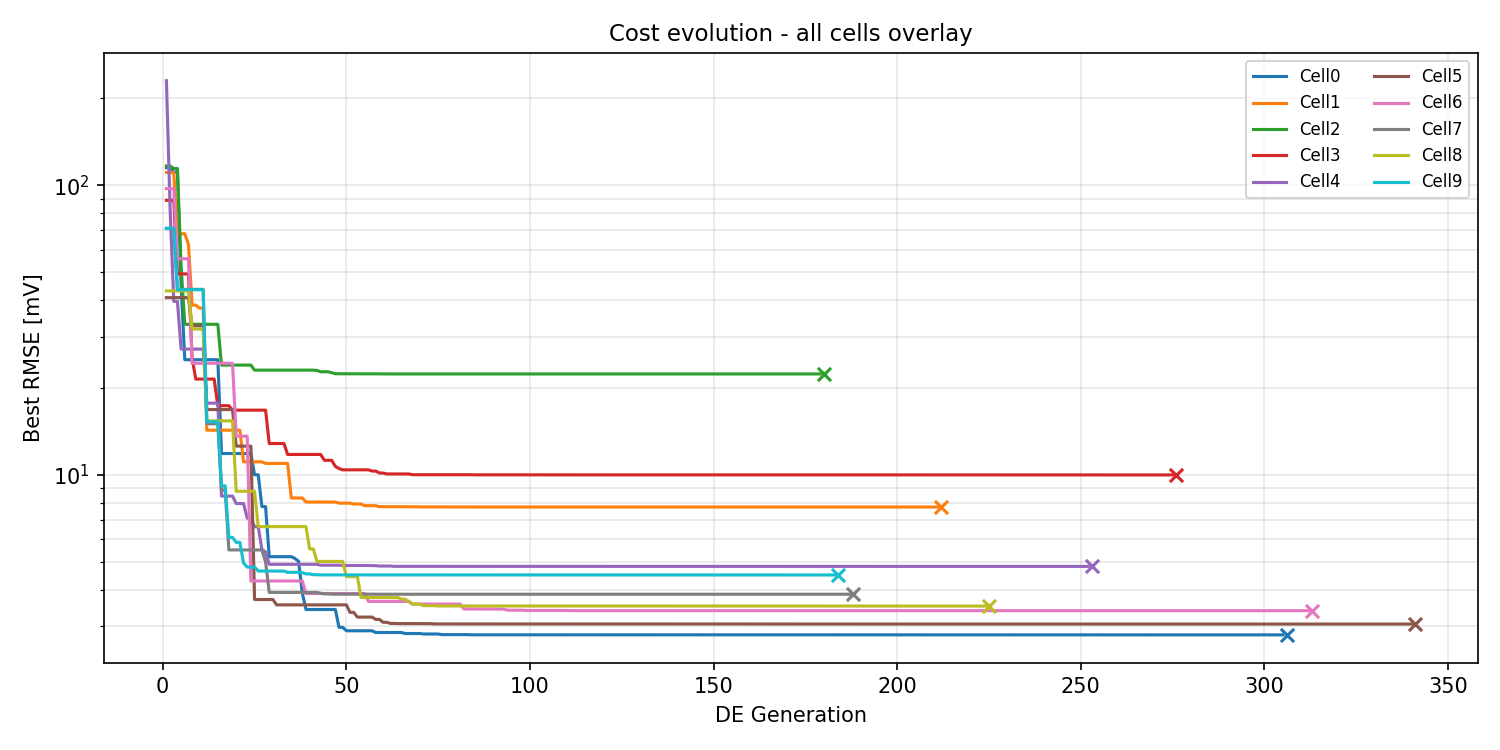
\includegraphics[width=\linewidth]{cost_evolution_overlay.png}
        \column{0.5\textwidth}
        \begin{itemize}
            \item Most cells converge within \textbf{50 generations}
            \item Cell\,2 stagnates at 22\,mV — hardest to fit
            \item L-BFGS-B polish gives negligible further gain
            \item Cells 1, 3 plateau $>$ 7\,mV — model mismatch
        \end{itemize}
    \end{columns}
\end{frame}

\begin{frame}{V--I Fits: All 10 Cells — Experiment 15}
    \begin{center}
        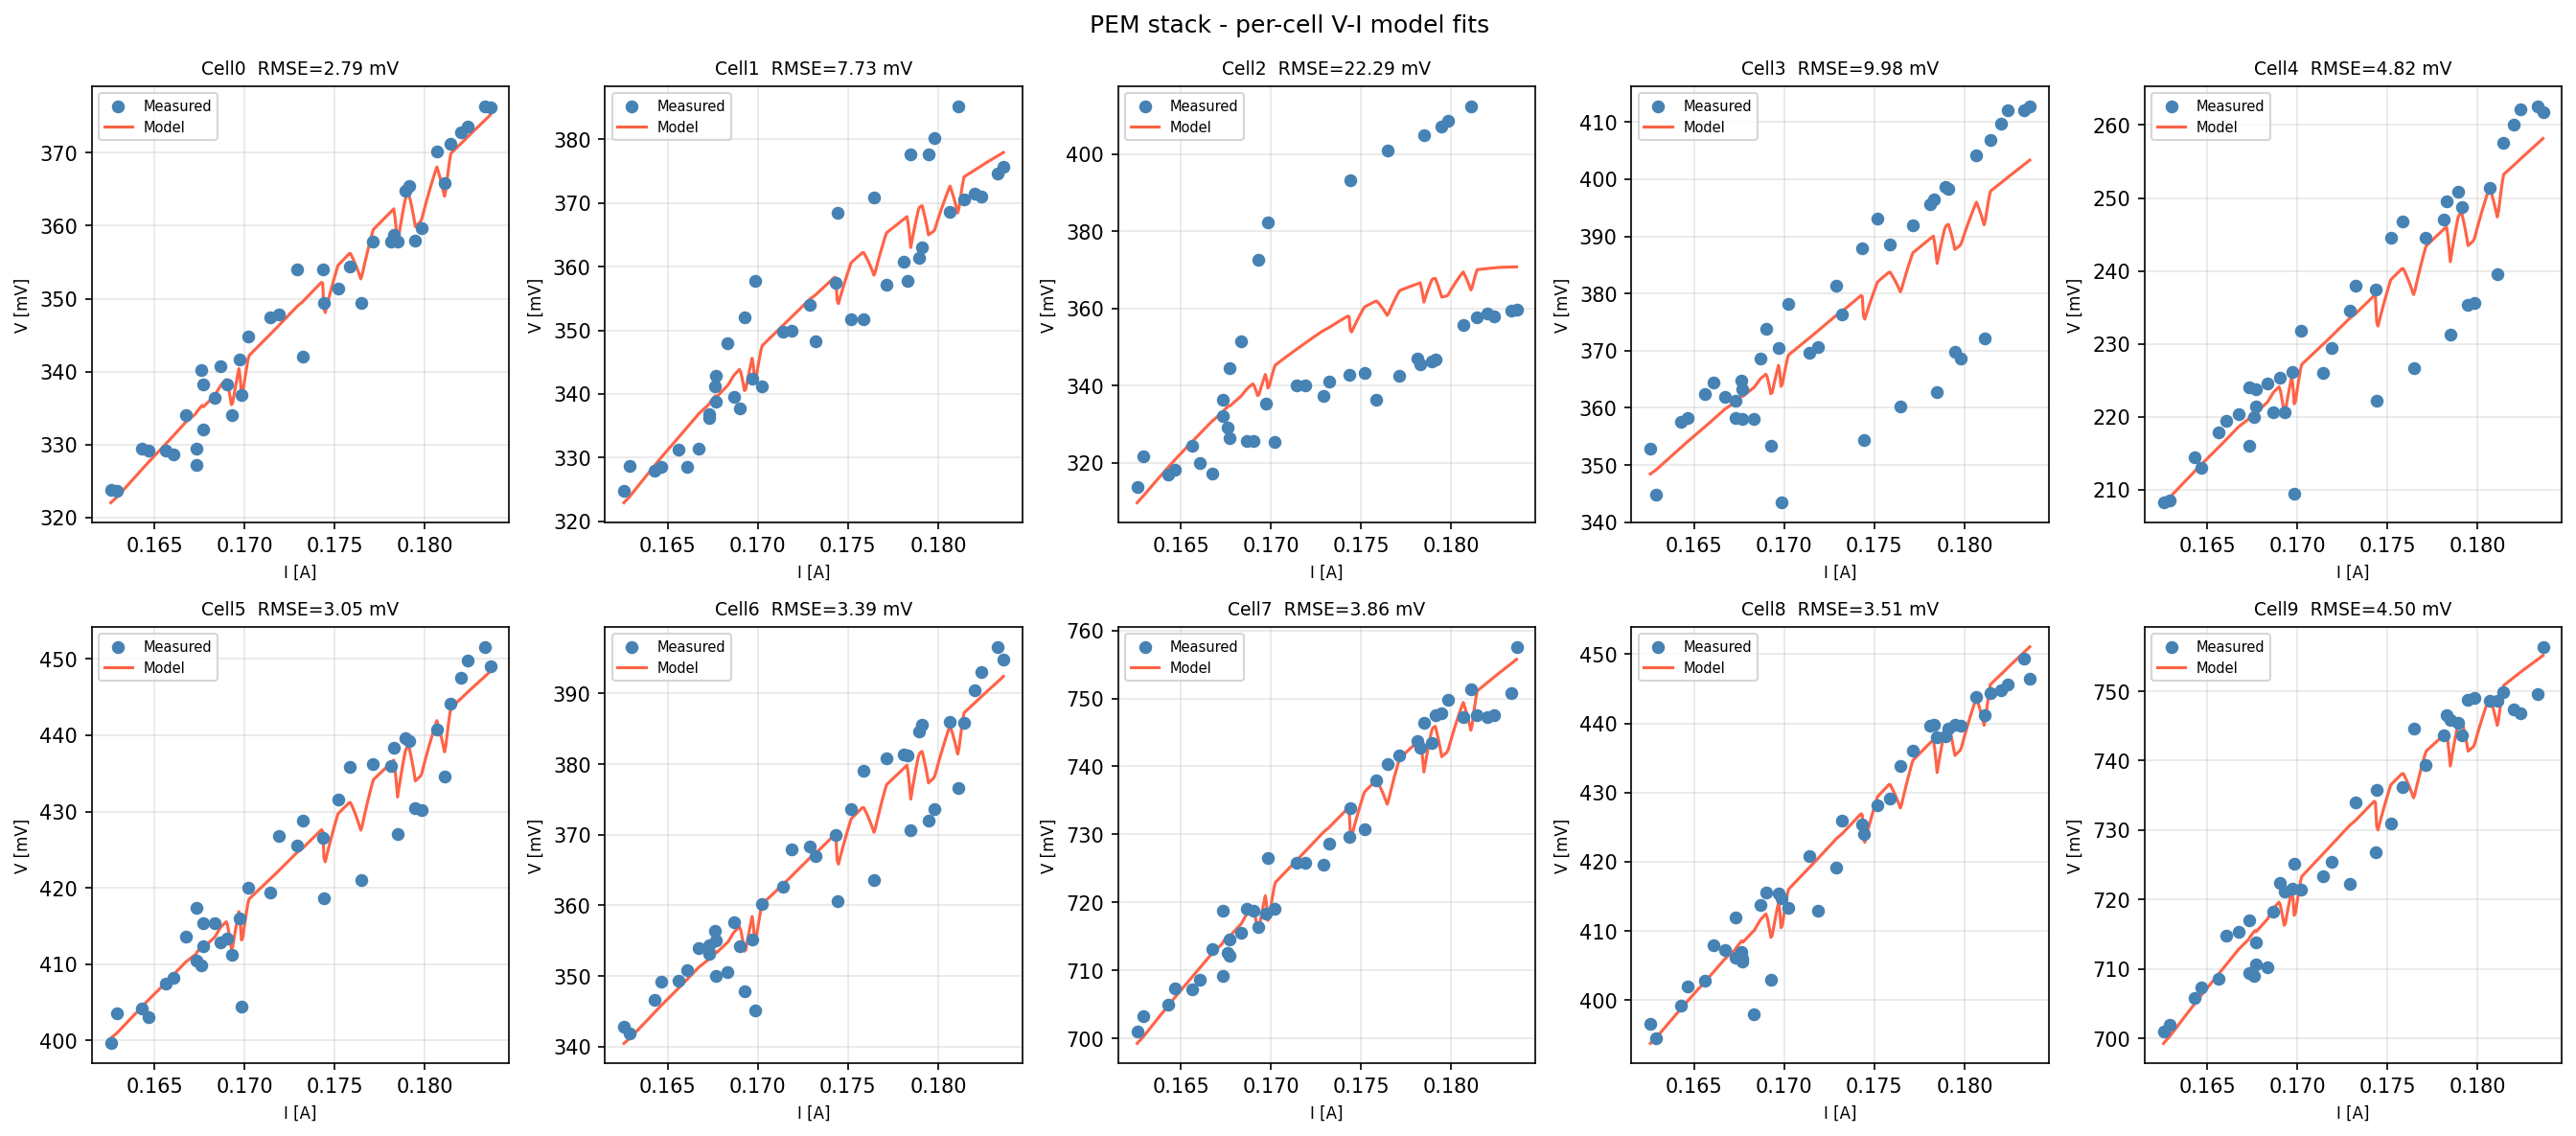
\includegraphics[width=0.92\linewidth]{all_cells_overview.png}
    \end{center}
\end{frame}

\begin{frame}{V--I Fits: All 10 Cells — Experiment 19}
    \begin{center}
        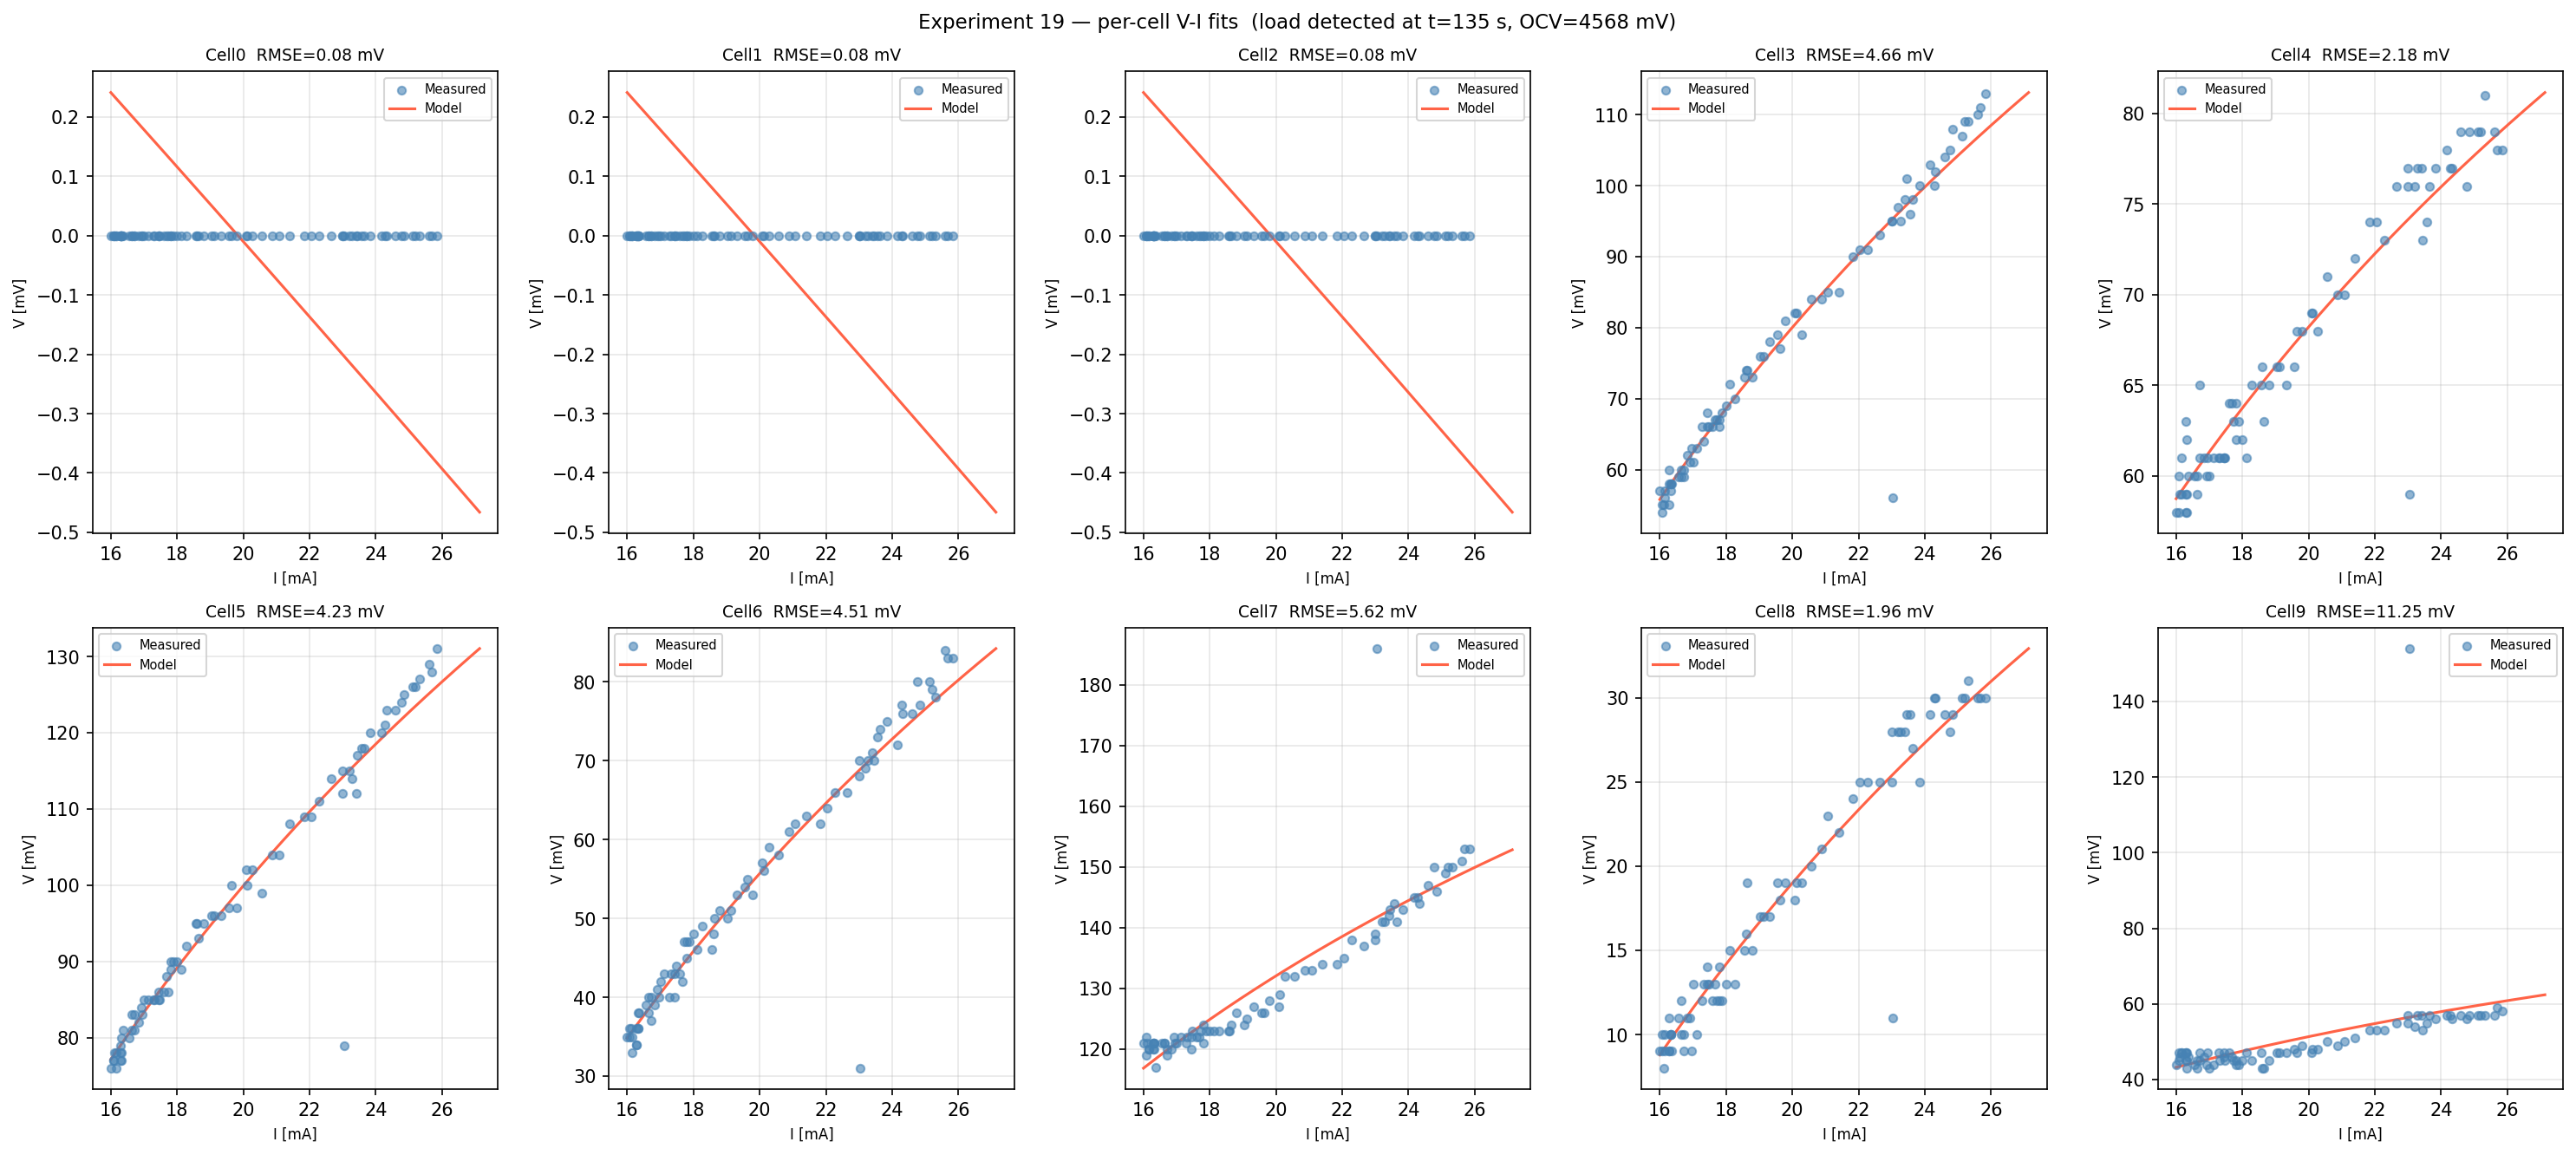
\includegraphics[width=0.92\linewidth]{all_cells_overview_exp19.png}
    \end{center}
\end{frame}

\begin{frame}{Tuned Parameters \& RMSE}
    \begin{center}
    \small
    \begin{tabular}{lrrrrrrr}
        \toprule
        Cell & RMSE (mV) & $\xi_1$ & $\xi_2$ & $\xi_3$ & $\xi_4$ & $B$ & $c$ \\
        \midrule
        Cell0 &  2.8 & $-0.884$ & $1.06\!\times\!10^{-2}$ & $5.0\!\times\!10^{-4}$ & $-1.26\!\times\!10^{-3}$ & $\approx 0$ & $\approx 0$ \\
        Cell1 &  7.7 & $-7.457$ & $1.11\!\times\!10^{-3}$ & $-1.0\!\times\!10^{-3}$ & $-3.32\!\times\!10^{-3}$ & $0.305$ & $\approx 0$ \\
        Cell2 & 22.3 & $ 1.350$ & $1.87\!\times\!10^{-3}$ & $1.3\!\times\!10^{-3}$ & $-8.07\!\times\!10^{-3}$ & $1.003$ & $1.1\!\times\!10^{-6}$ \\
        Cell3 & 10.0 & $-2.885$ & $1.30\!\times\!10^{-3}$ & $-4.6\!\times\!10^{-4}$ & $-1.30\!\times\!10^{-3}$ & $\approx 0$ & $\approx 0$ \\
        Cell4 &  4.8 & $-7.935$ & $1.12\!\times\!10^{-2}$ & $-8.1\!\times\!10^{-4}$ & $-1.18\!\times\!10^{-3}$ & $\approx 0$ & $\approx 0$ \\
        Cell5 &  3.0 & $-7.967$ & $3.28\!\times\!10^{-3}$ & $-1.3\!\times\!10^{-3}$ & $-1.14\!\times\!10^{-3}$ & $\approx 0$ & $\approx 0$ \\
        Cell6 &  3.4 & $ 1.354$ & $2.53\!\times\!10^{-2}$ & $1.9\!\times\!10^{-3}$ & $-1.23\!\times\!10^{-3}$ & $\approx 0$ & $\approx 0$ \\
        Cell7 &  3.9 & $-6.255$ & $6.39\!\times\!10^{-3}$ & $-5.2\!\times\!10^{-4}$ & $-2.53\!\times\!10^{-3}$ & $0.181$ & $\approx 0$ \\
        Cell8 &  3.5 & $-0.655$ & $2.72\!\times\!10^{-3}$ & $1.1\!\times\!10^{-4}$ & $-1.65\!\times\!10^{-3}$ & $0.043$ & $\approx 0$ \\
        Cell9 &  4.5 & $-3.032$ & $9.24\!\times\!10^{-3}$ & $3.1\!\times\!10^{-4}$ & $-2.84\!\times\!10^{-3}$ & $0.229$ & $\approx 0$ \\
        \bottomrule
    \end{tabular}
    \end{center}
\end{frame}

% ─────────────────────────────────────────────────────────────────────────────
% ─────────────────────────────────────────────────────────────────────────────
\section{Simulation vs Experiment}

% ── Experiment 15 ─────────────────────────────────────────────────────────────
\begin{frame}{Exp\,15 — Per-Cell Voltage: Measured vs Simulated}
    \begin{center}
        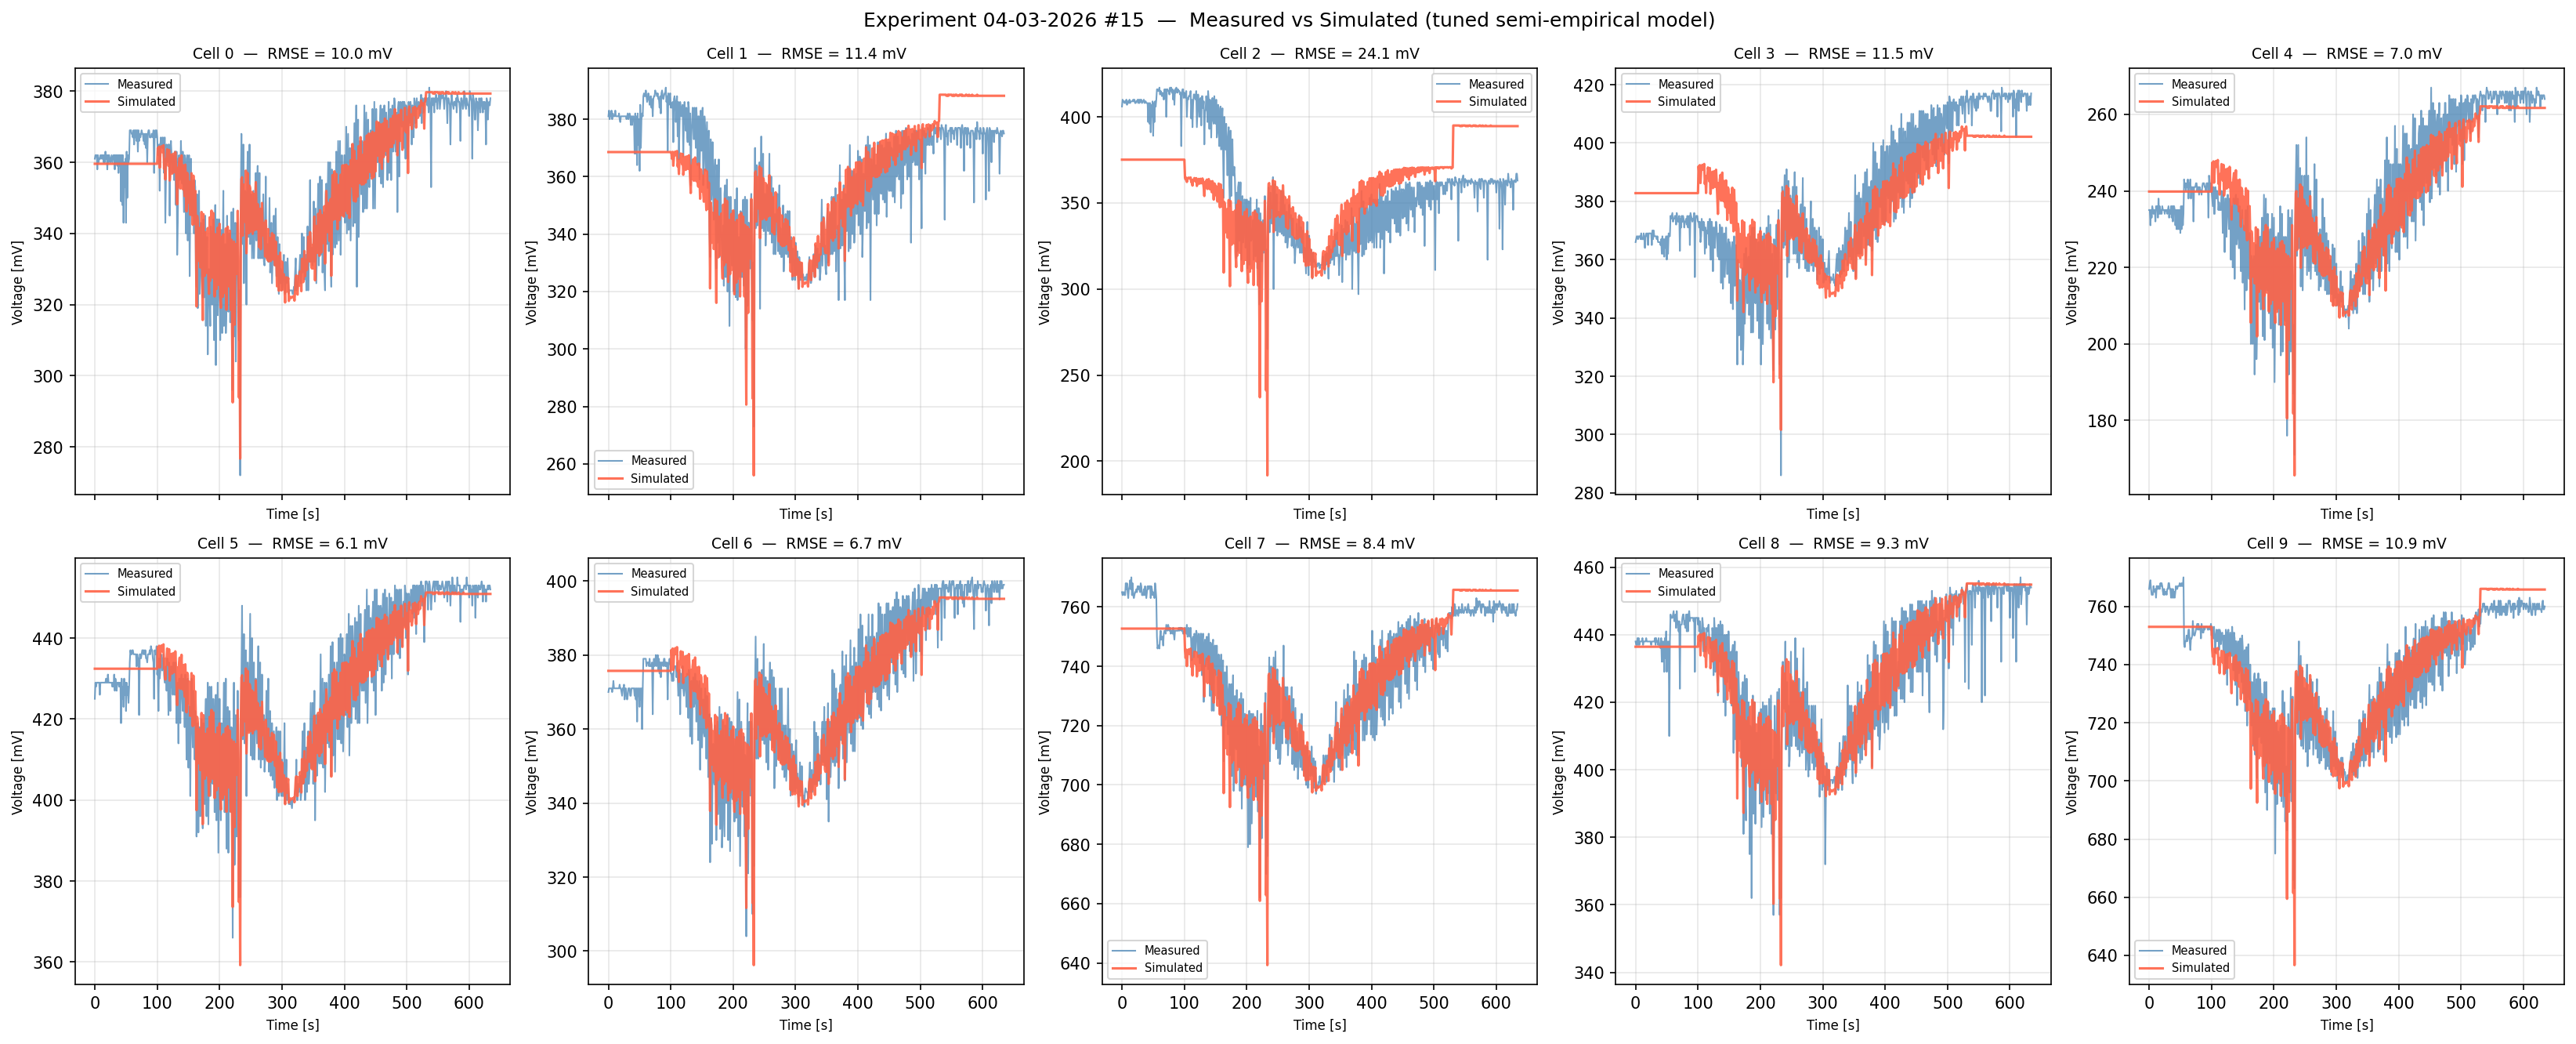
\includegraphics[width=0.95\linewidth]{comparison_exp15_cells.png}
    \end{center}
    \vspace{-0.4em}
    {\small OCV region: Nernst model (T\textsubscript{eff} fitted per cell). \quad
           Loaded region: tuned semi-empirical model. \quad Mean RMSE\,=\,10.6\,mV}
\end{frame}

\begin{frame}{Exp\,15 — Stack Voltage \& Load Current}
    \begin{center}
        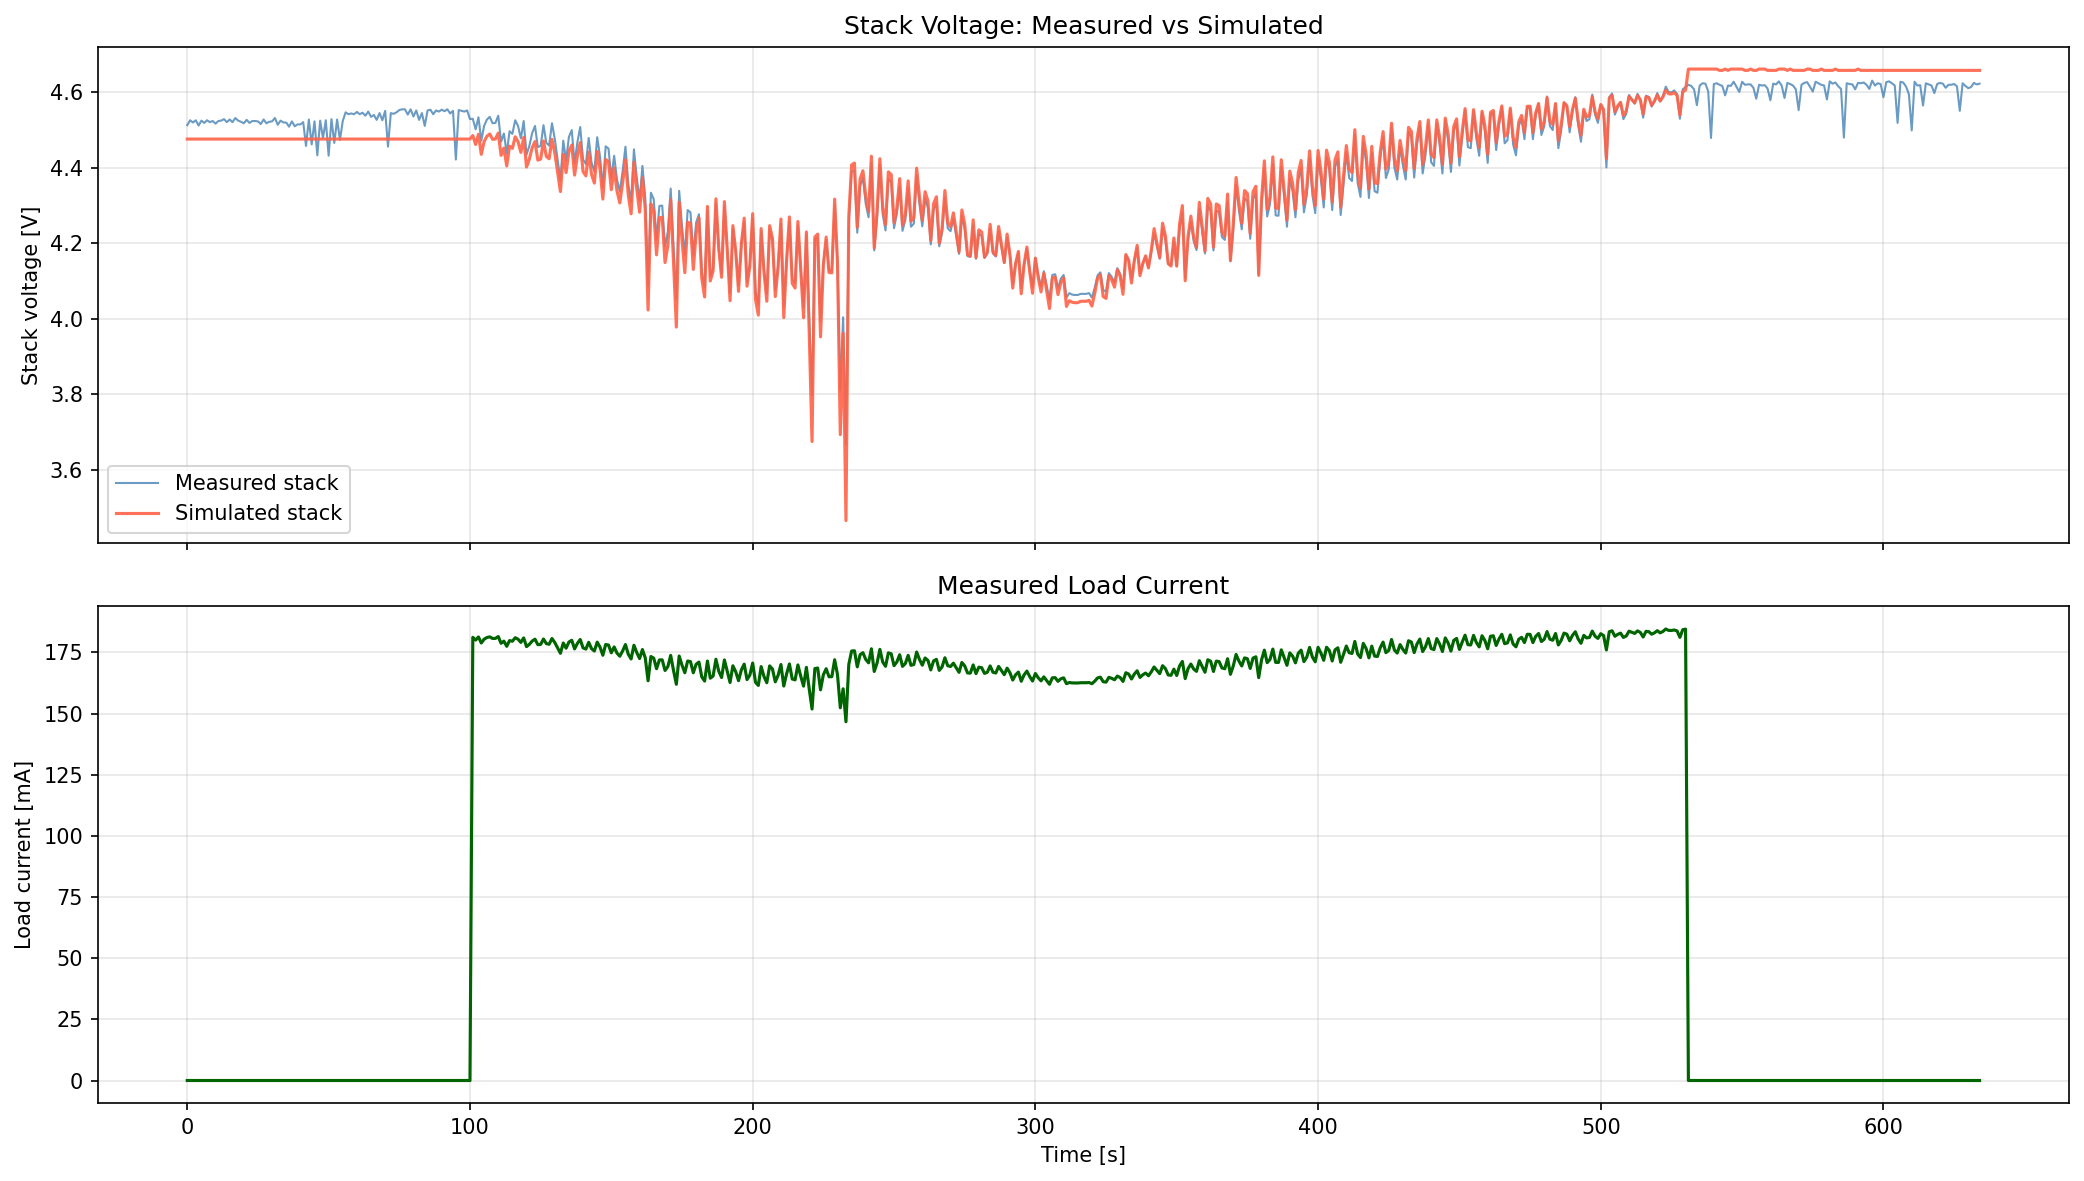
\includegraphics[width=0.88\linewidth]{comparison_exp15_stack.png}
    \end{center}
\end{frame}

\begin{frame}{Exp\,15 — Per-Cell Voltage Error}
    \begin{center}
        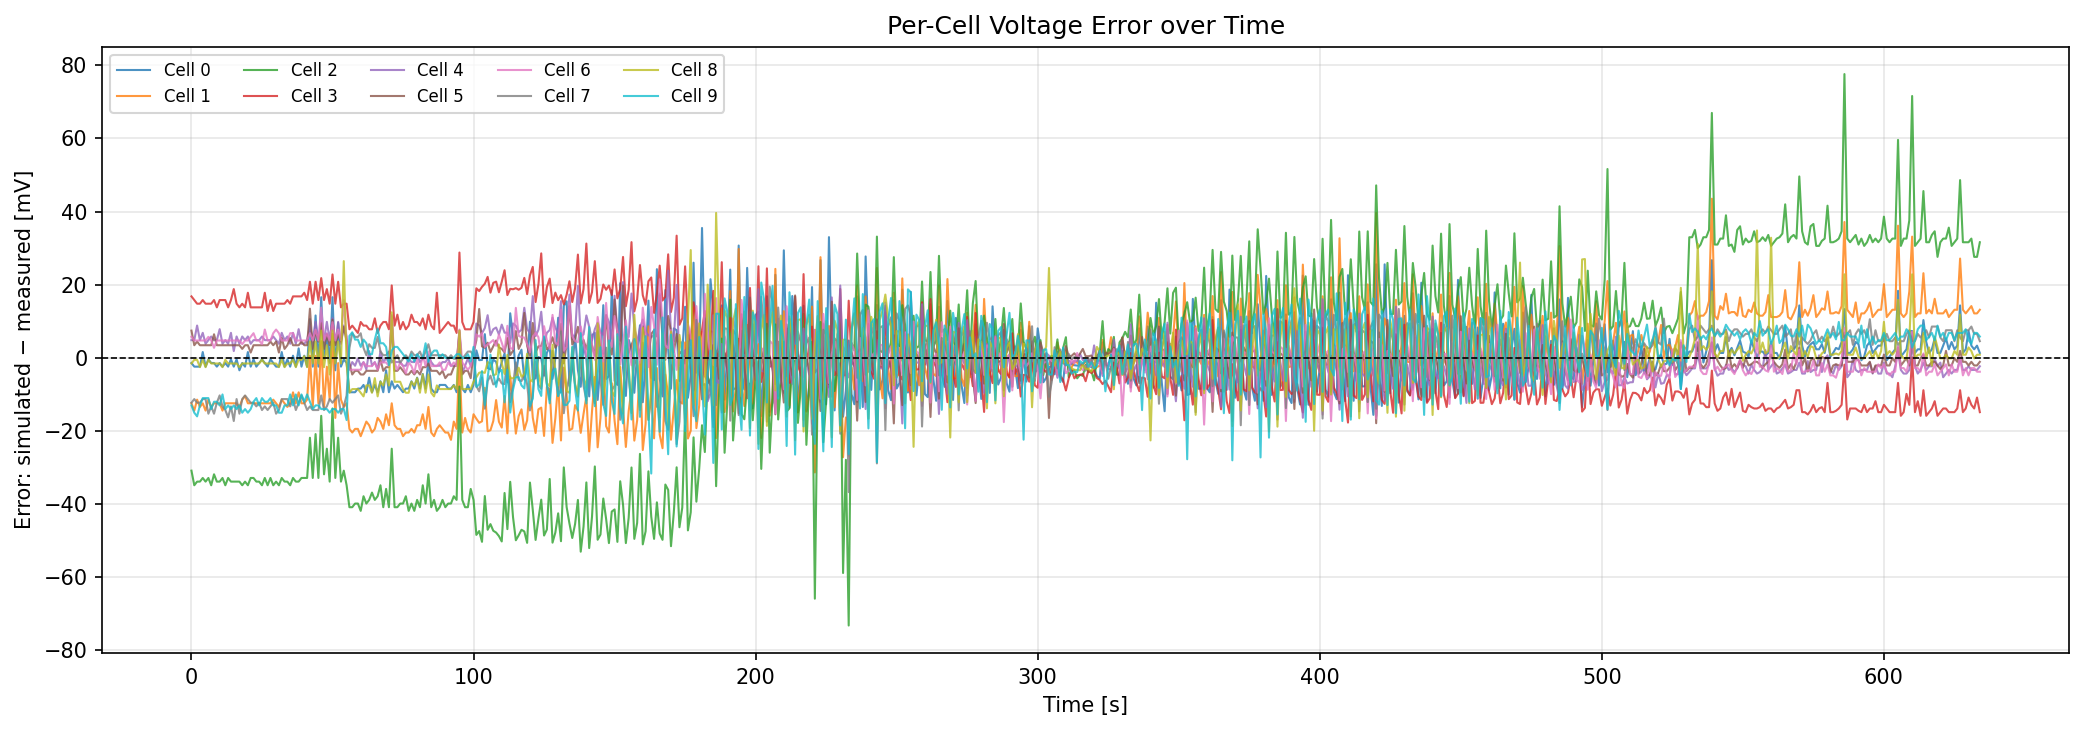
\includegraphics[width=0.88\linewidth]{comparison_exp15_error.png}
    \end{center}
    {\small Error\,$=$\,simulated\,$-$\,measured. Positive bias in degraded cells (Cell\,2).}
\end{frame}

% ── Experiment 19 ─────────────────────────────────────────────────────────────
\begin{frame}{Exp\,19 — Per-Cell Voltage: Measured vs Simulated}
    \begin{center}
        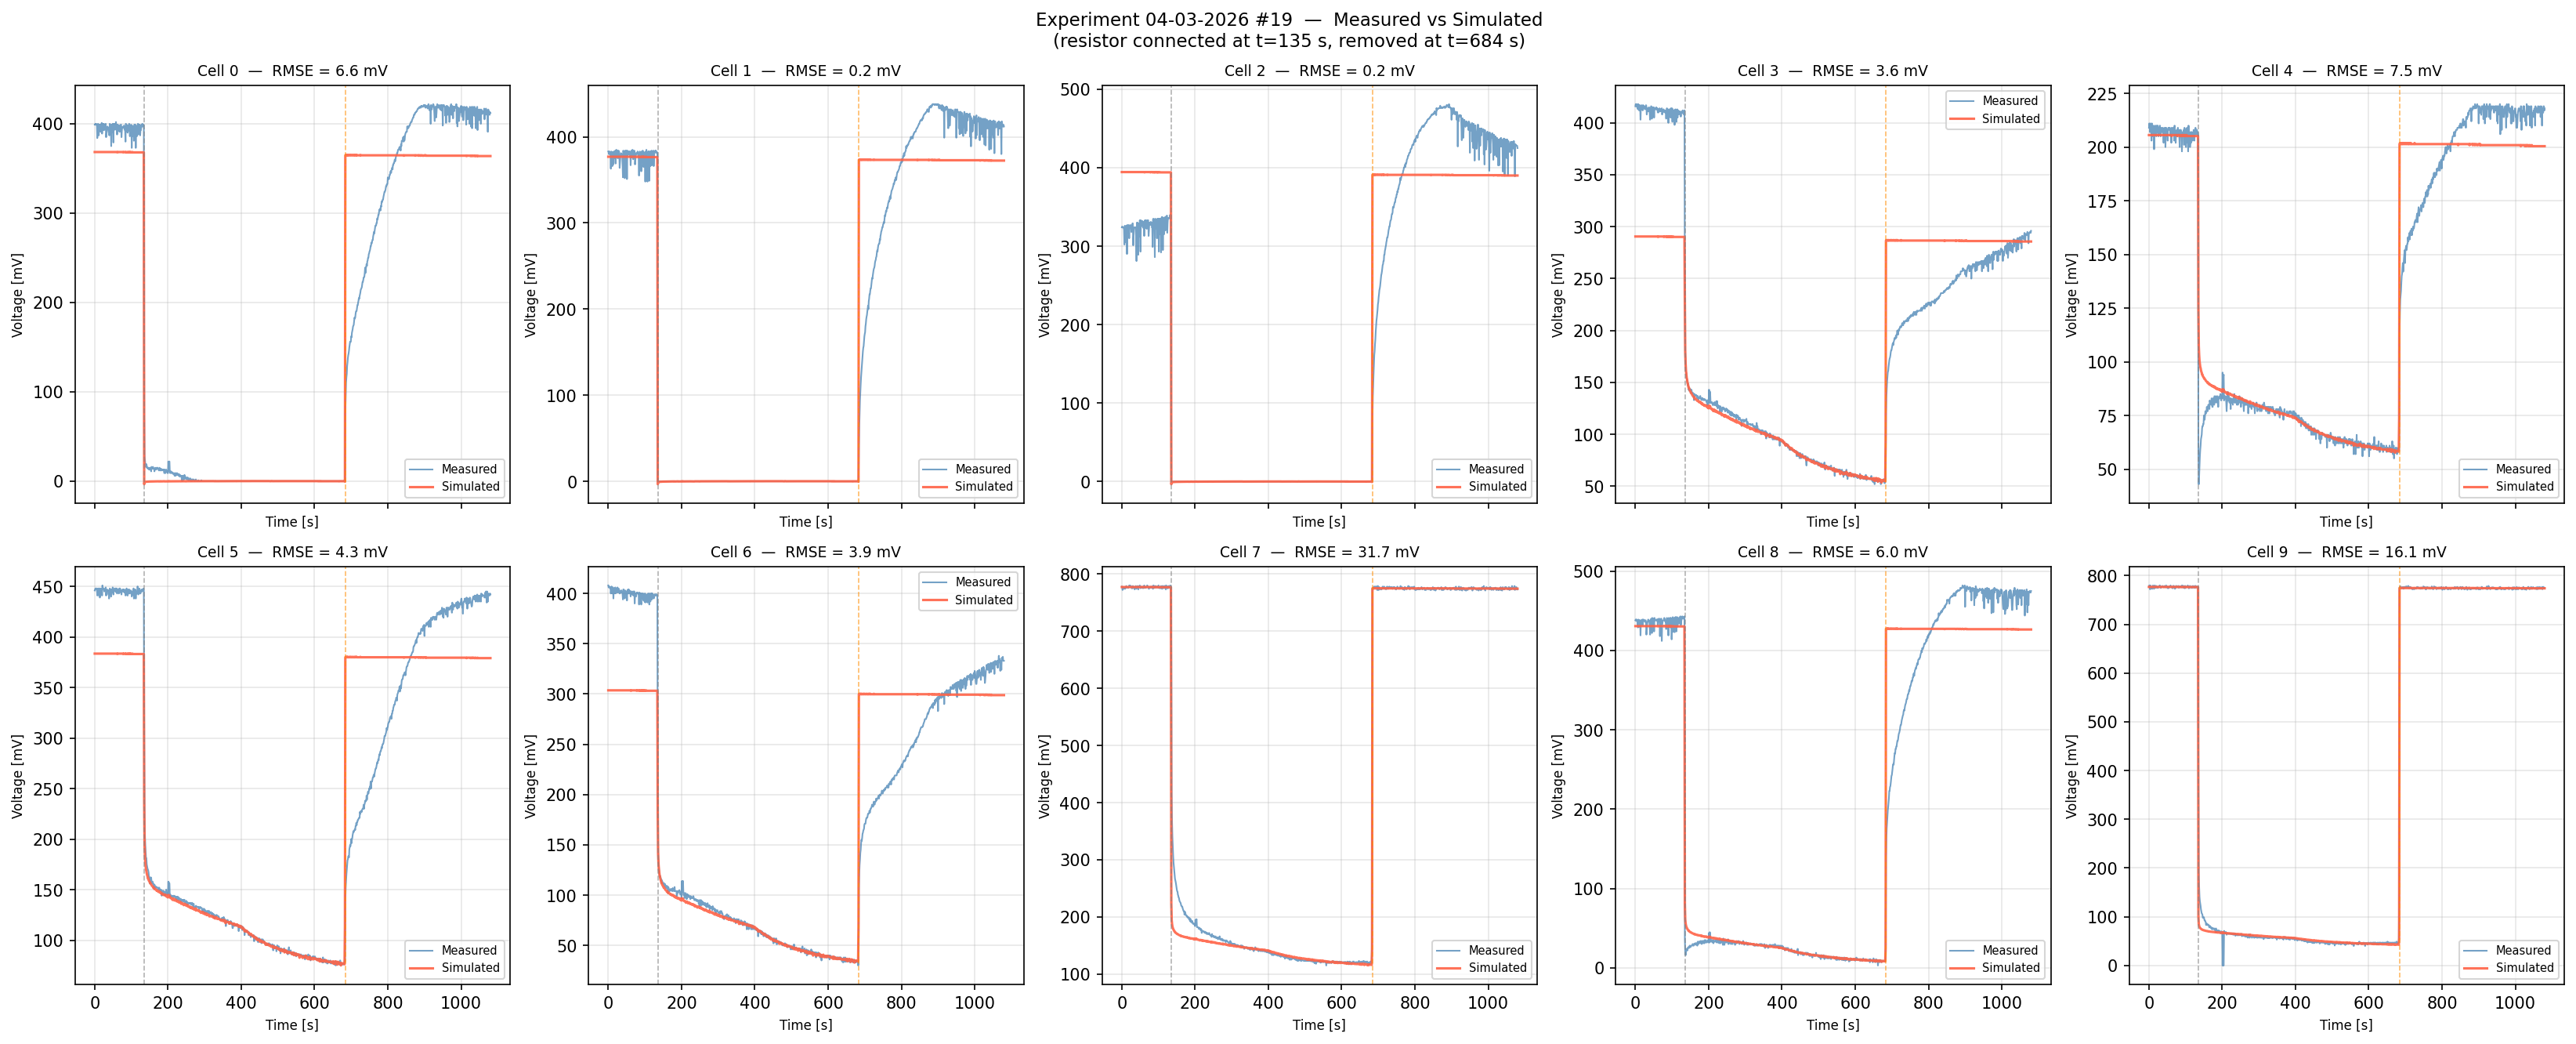
\includegraphics[width=0.95\linewidth]{comparison_exp19_cells.png}
    \end{center}
    \vspace{-0.4em}
    {\small Load applied at $t=135$\,s via 25\,$\Omega$ resistor, removed at $t=684$\,s ($I = 0$ after removal). \quad
           Cells\,0,\,1,\,2\,\&\,8 collapse to $\approx$\,0\,V (hardware degradation). \quad Mean RMSE\,=\,8.0\,mV}
\end{frame}

\begin{frame}{Exp\,19 — Stack Voltage, Current \& Pressure}
    \begin{center}
        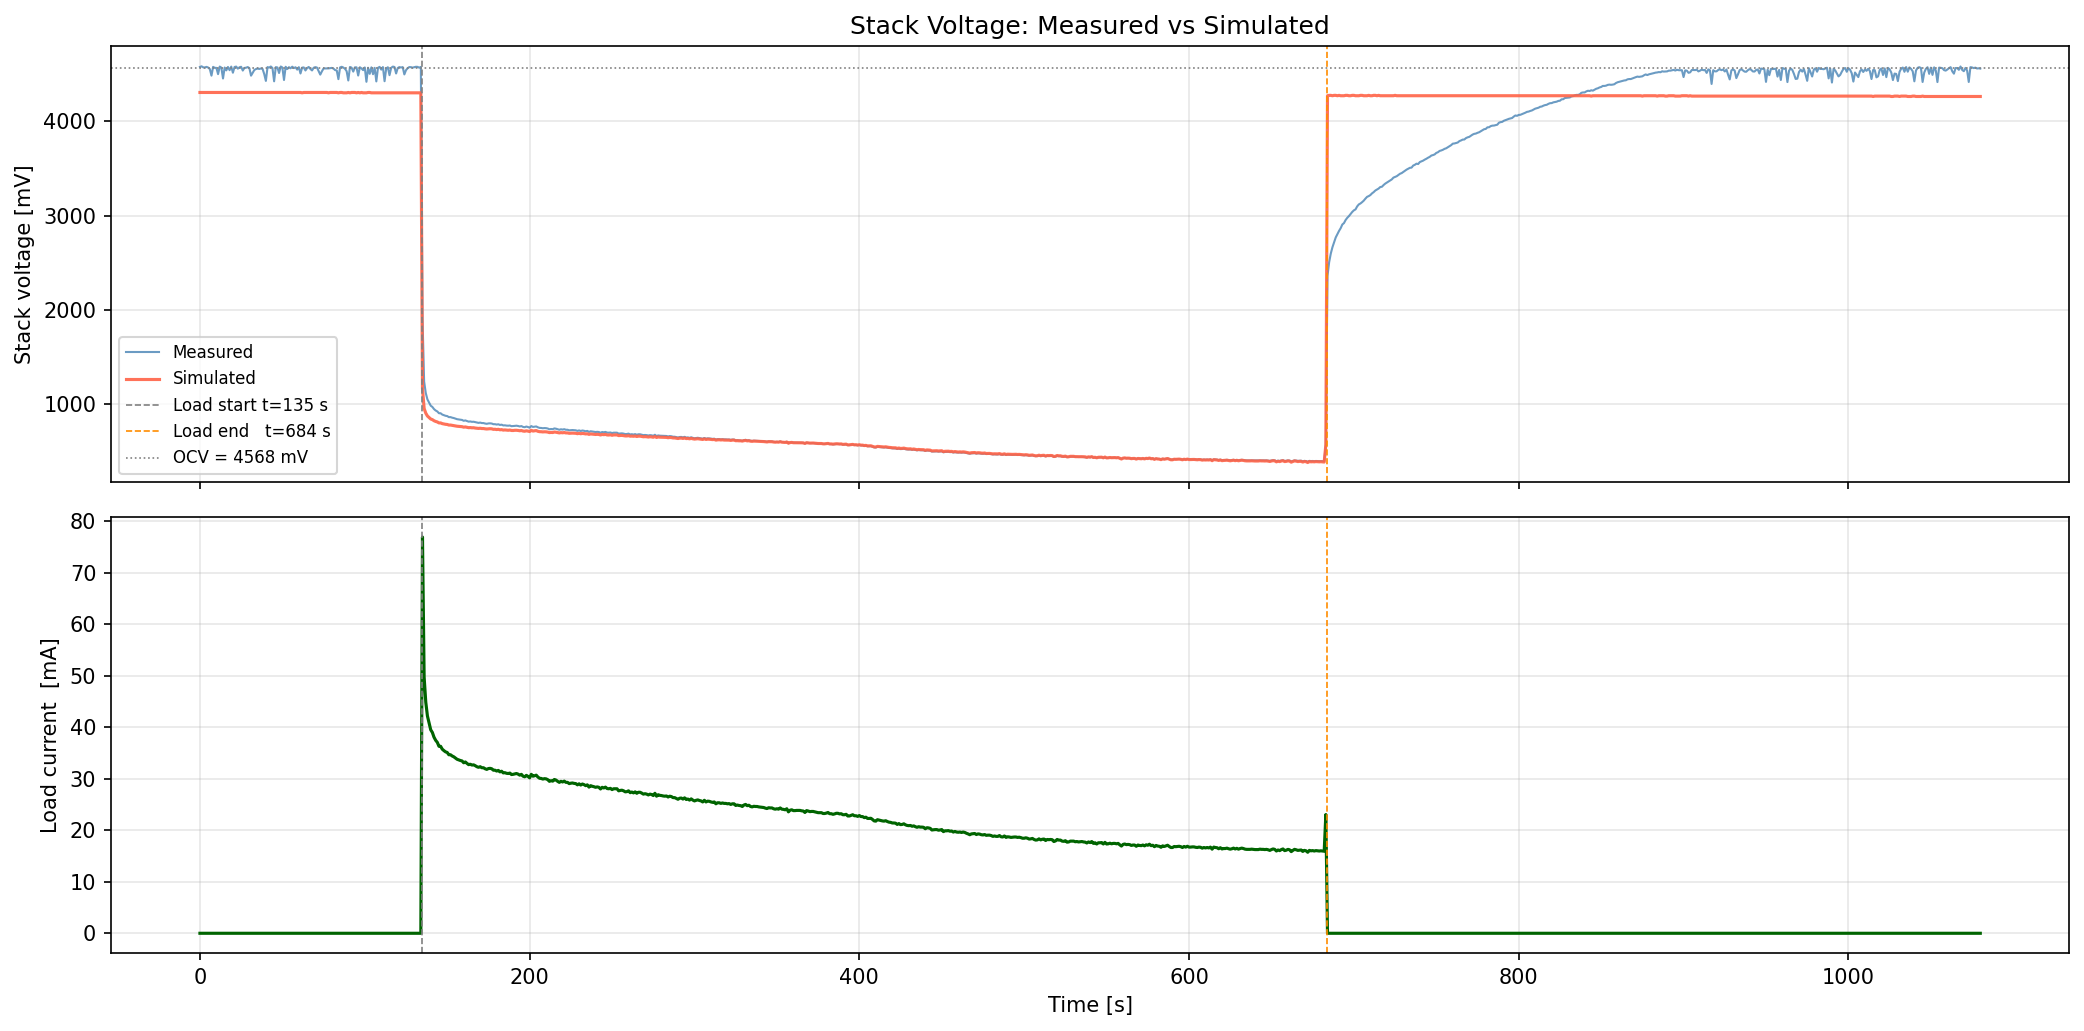
\includegraphics[width=0.82\linewidth]{comparison_exp19_stack.png}
    \end{center}
\end{frame}

\begin{frame}{Exp\,19 — Per-Cell Voltage Error}
    \begin{center}
        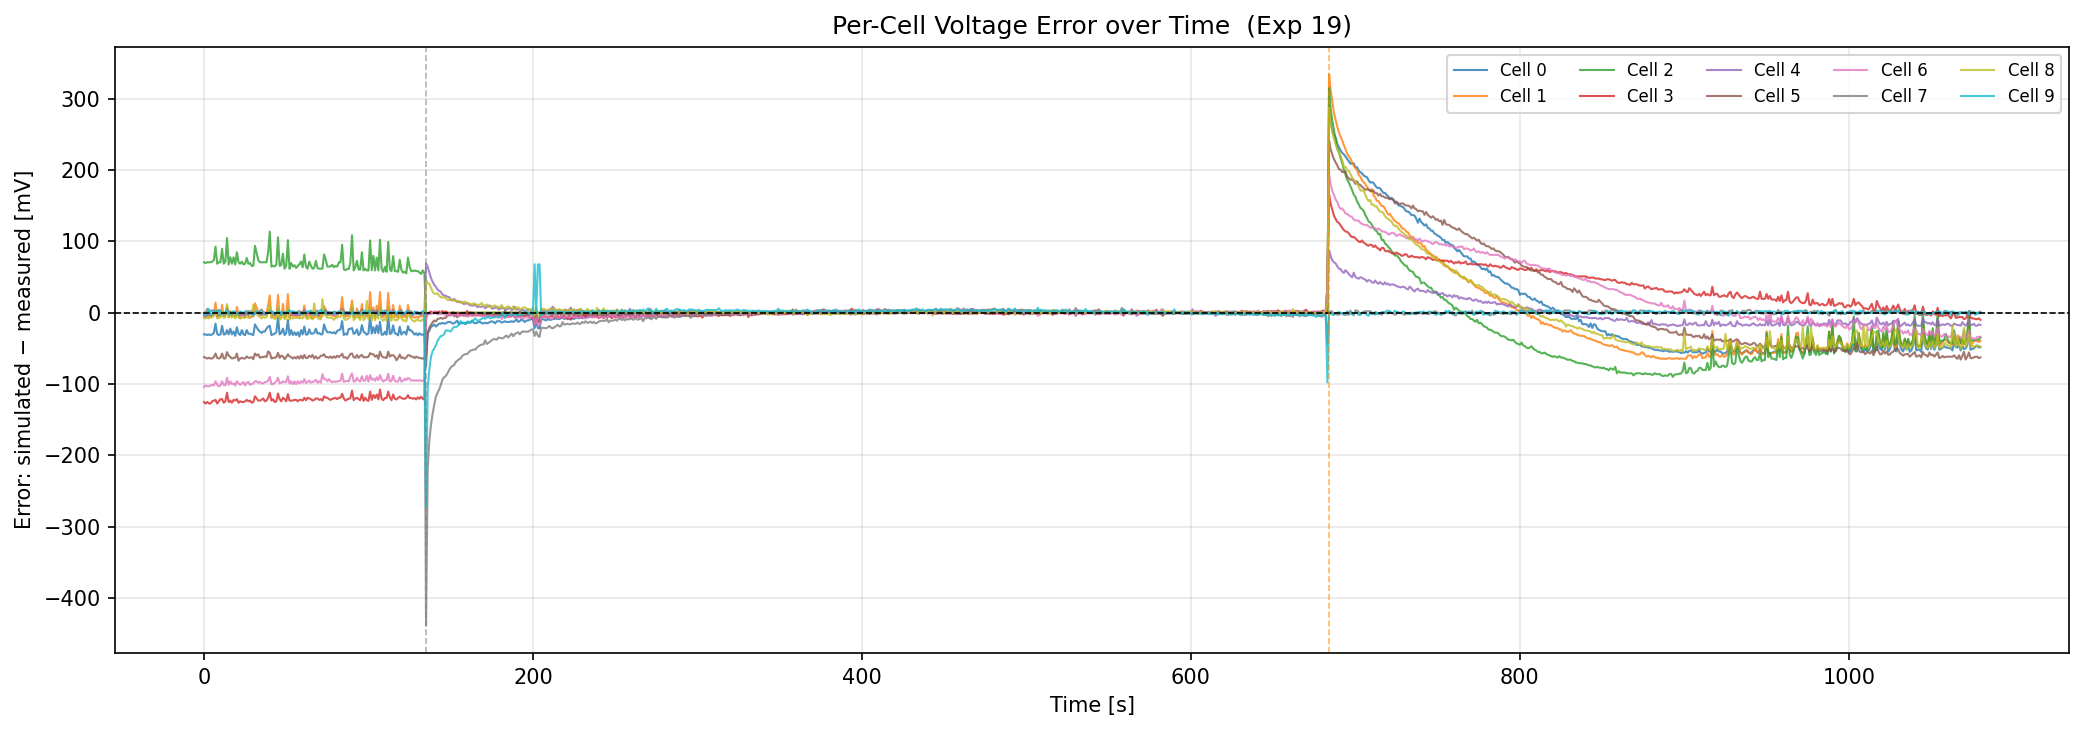
\includegraphics[width=0.88\linewidth]{comparison_exp19_error.png}
    \end{center}
    {\small Large errors for degraded cells (0, 1, 2, 8) — model cannot capture hardware failure.}
\end{frame}

% ─────────────────────────────────────────────────────────────────────────────
\section{Conclusion}

\begin{frame}{Conclusion}
    \begin{itemize}
        \item Physical principles → semi-empirical voltage model → reduced state-space system
        \item 6 parameters tuned per cell using real experimental V--I data
        \item 8 out of 10 cells fitted with RMSE $\leq$ 5\,mV
        \item Cell\,2 (22\,mV) and Cell\,3 (10\,mV) — degradation not fully captured by the model
        \item Concentration loss ($B > 0$) in Cells 1, 2, 7, 8, 9 → mass-transport limitations
        \item Parameters exported to \texttt{tuned\_params.csv} for Simulink/MATLAB integration
    \end{itemize}
\end{frame}

\end{document}

